\section{Containers}

\begin{frame}{Importance of Containers}
\centering
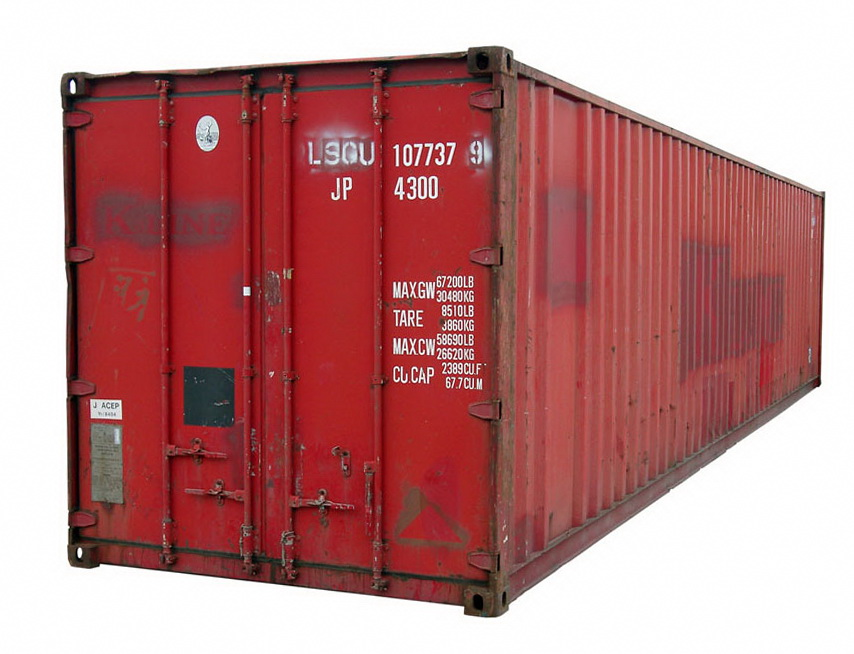
\includegraphics[width=0.7\textwidth]{images/shipping_container}
\end{frame}

\begin{frame}{Before Containerization}
\begin{columns}[c]
\begin{column}{0.5\textwidth}
\begin{itemize}
\item Goods had to be loaded and unloaded individually
\item Inefficient - it was not uncommon to spend more time loading and loading goods than transporting them
\item Insecure - goods had be handled by many people, increasing the chance for loss and theft
\item Inaccessible - Long distance shipping only available to the wealthy 
\end{itemize}
\end{column}
\begin{column}{0.5\textwidth}
\centering
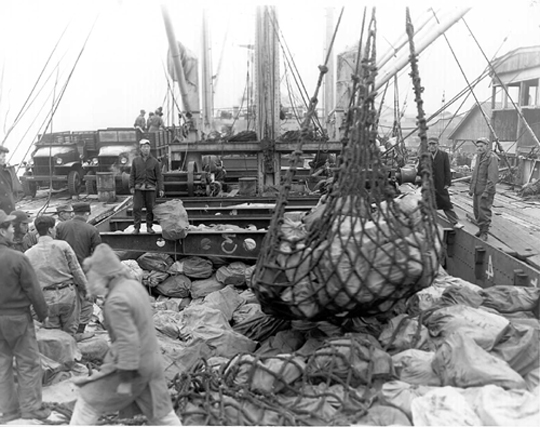
\includegraphics[width=0.85\textwidth]{images/old_ship_unloading}
\end{column}
\end{columns}
\end{frame}

\begin{frame}{After Containerization}
\begin{columns}[c]
\begin{column}{0.5\textwidth}
\begin{itemize}
\item Standardized - containers are all the same size and weight allowances
\item Efficient - containers are easy to load and unload and transfer to other modes of transportation
\item Secure - goods may be secured in containers from source to final destination
\item Available - cost effective to ship goods across the world
\end{itemize}
\end{column}
\begin{column}{0.5\textwidth}
\centering
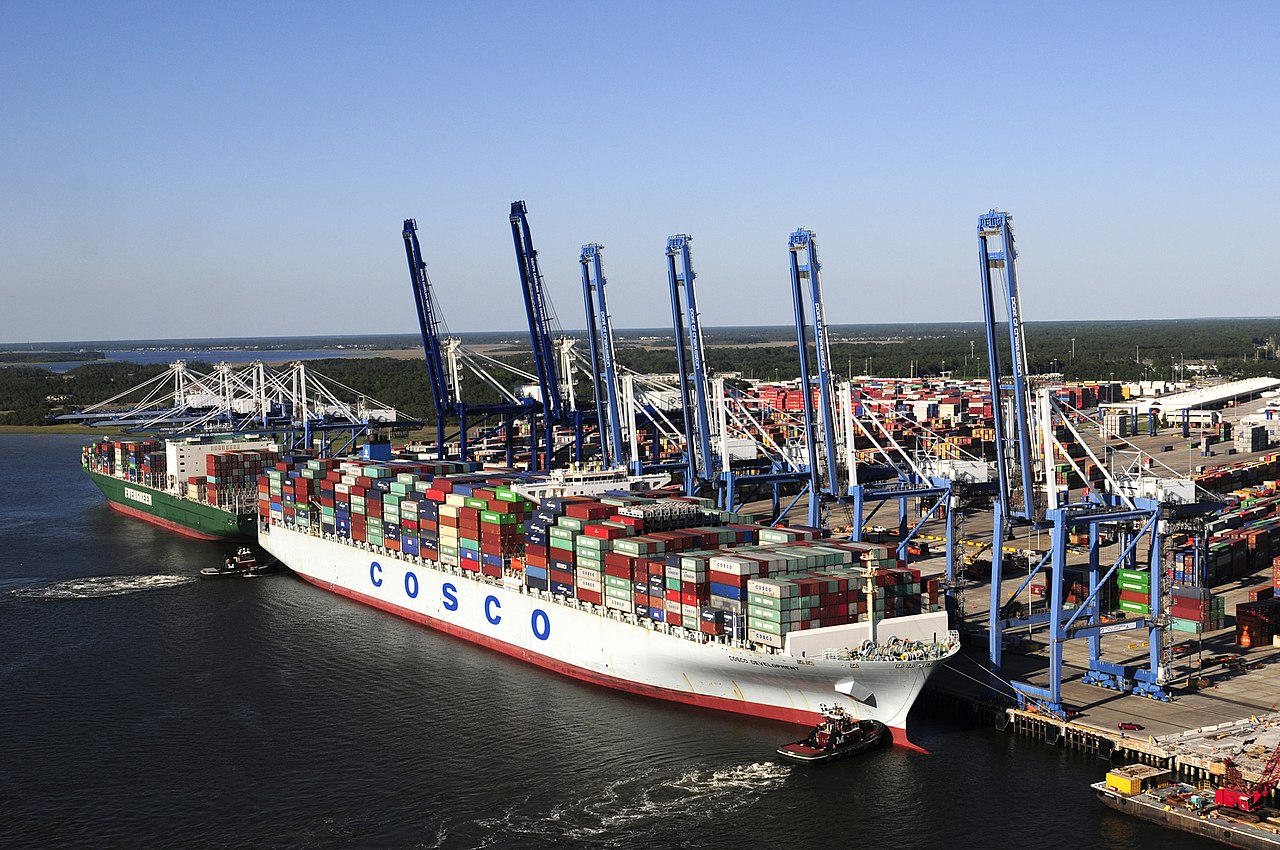
\includegraphics[width=0.85\textwidth]{images/cargo_ship}
\end{column}
\end{columns}

\end{frame}

\begin{frame}{Common Issues with Software Stacks}
\begin{itemize}
\item My software doesn’t build on this system...
\item I’m missing dependencies...
\item I need version 1.3.2 but this system has version 1.0.2..
\item I need to re-run the exact same thing 12 months from now...
\item I want to run this exact same thing somewhere else...
\item I want my collaborators to have the same exact software as me...
\item I’ve heard about these Containers, can I just run that?
\item Can I run docker on this HPC system?
\end{itemize}
\end{frame}

\begin{frame}{What about computing?}
\begin{itemize}
\item It's common to run on multiple systems with different requirements
\item We would like to avoid installing the same sets of software again and again
\item We would like other people to run our software without our help
\item We would like to preserve a known configuration that our software works in
\end{itemize}
\end{frame}

\begin{frame}{Possible Solution: Containers}
\begin{itemize}
\item What are Containers?
\item Uses a combination of Kernel ``cgroups'' and ``namespaces'' to create isolated environments
\item Long history of containers Solaris Zones (2005), LXC(2008), LMCTFY/Google and then Docker(2013).
\item Entire ecosystem has grown around containers including open standards and governance.
\end{itemize}
\end{frame}

\begin{frame}{Possible Solution: Containers}
\begin{itemize}
\item A lightweight collection of executable software that encapsulates
everything needed to run an application
\begin{itemize}
\item Minus the OS kernel
\item Based on Linux only
\end{itemize}
\item Processes and all user-level software is isolated
\item Creates a portable* software ecosystem
\item Think \mintinline{sh}{chroot} on steroids
\item Docker is the most common tool today
\begin{itemize}
\item Available on all major platforms
\item Widely used in industry
\item Integrated container registry via Dockerhub
\end{itemize}
\end{itemize}
\end{frame}

\begin{frame}{Containers Overview}
\begin{itemize}
\item Containers offer the ability to run fully customized software stacks,
\textit{e.g.} based on different Linux distributions and versions
\item Containers are not virtual machines, where an entire hardware platform is
virtualized, rather containers share a common kernel and access to physical
hardware resources
\end{itemize}
\end{frame}

\begin{frame}{Hypervisors and Containers}
\begin{itemize}
\item Type 1 hypervisors insert layer below host OS
\item Type 2 hypervisors work as or within the host OS
\item Containers do not abstract hardware, instead provide ``enhanced chroot'' to
create isolated environment using a common kernel
\item Location of abstraction can have impact on performance
\item All enable custom software stacks on existing hardware
\end{itemize}
\end{frame}

\begin{frame}{Hypervisors and Containers}
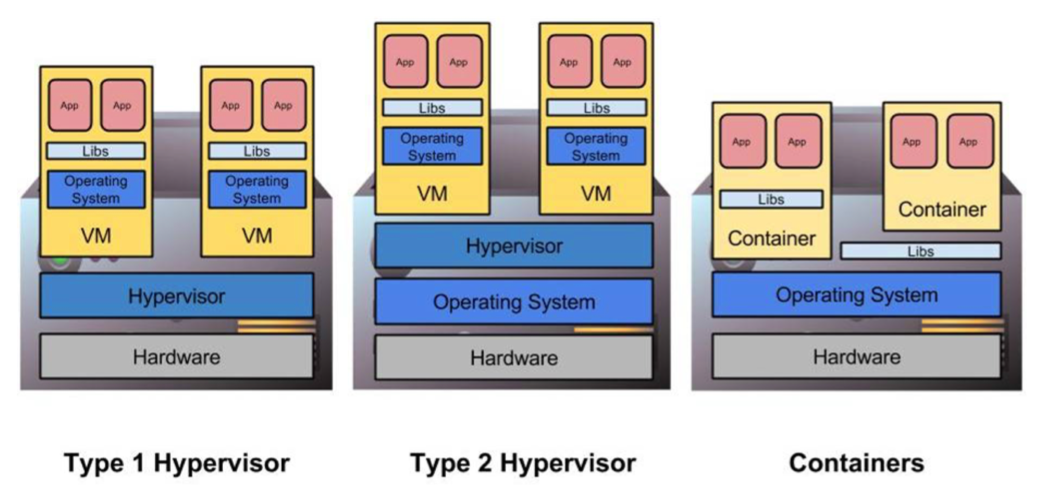
\includegraphics[height=0.8\textheight]{images/hypervisors_vs_containers.png}
\end{frame}

\begin{frame}{Container Benefits}
\begin{description}
\item[Performant] Containers can perform at near native performance.
\item[Flexible] Install (almost) any software you need.
\item[Reproducible] Define complex software environments that are verifiable.
\item[Compatible] Built on open standards that works on all major Linux distributions.
\item[Portable] Build once and run (almost) anywhere.
\end{description}
\end{frame}

\begin{frame}{Container Limitations}
\begin{description}
\item[Hardware] Containers are limited to the same CPU architecture
(x86\_64, ARM, Power, etc.) and binary formats
\item[Software] Requires glibc and kernel compatibility between host and
container. Other kernel level APIs may also need to be compatible (e.g.
CUDA/GPU drivers, network drivers, etc.)
\item[Filesystem] Paths can be different when viewed from inside or outside of
a container
\end{description}
\end{frame}

\begin{frame}{Nomenclature}
\begin{description}
\item[Image] A read-only template that defines how to create a container
\item[Container] An instantiation of an image, a running instance
\item[Container Runtime] Tool or service to execute and manage containers
\item[Registry] A service that is used to store and distribute images
\end{description}
\end{frame}

\begin{frame}{Docker and HPC}
\begin{itemize}
\item We don't allow direct Docker use on SMU HPC systems
\item Docker's security model is designed to support users "trusted" users running "trusted" containers (e.g. users who can escalate to root access)
\item Docker is not designed to support scripted / batch based workflows
\item Docker is not designed to support parallel applications
\end{itemize}
\end{frame}

\begin{frame}{Apptainer/Singularity Features}
\begin{itemize}
\item Containers are a single image file
\item No root owned daemon processes
\item User inside containers are the same as users outside the container (no contextual changes)
\item Supports shared, multi-user environments
\item Supports HPC hardware such as GPUs and Infiniband networks
\item Supports HPC applications like MPI
\end{itemize}
\end{frame}

\begin{frame}{Common Use Cases}
\begin{itemize}
\item Converting Docker containers to Apptainer/Singularity
\item Building and running software that require newer systems and libraries 
\item Running commercial software binaries that have specific requirements
\end{itemize}
\end{frame}

